%!TEX root = main.tex
\section{Results}

The Dieleman model was used for both sex and speaker classification. The results are presented below.

\begin{table}[H]
\centering
\begin{tabular}{r|c|c}
model & TIMIT & ELSDSR \\ \hline
                    Baseline & $0.354$ & $0.465$ \\
                    Logistic & $0.094 \pm 0.012$ & $0.030 \pm 0.007$ \\
                 GMM on MFCC & $0.192 \pm 0.024$ & $0.140 \pm 0.019$ \\
                    Dieleman & $0.093 \pm 0.012$ & $0.026 \pm 0.006$ \\
     Dieleman + Weight Decay & $0.114 \pm 0.013$ & $0.036 \pm 0.016$ \\
  Dieleman + Scale Invarient & $0.111 \pm 0.015$ & $0.022 \pm 0.006$ \\
 Dieleman + Offset Invarient & $0.107 \pm 0.008$ & $0.027 \pm 0.014$ \\
\end{tabular}
\caption{misclassification rate for sex classification with $95\%$ confidence internal.}
\end{table}

\begin{table}[H]
\centering
\begin{tabular}{r|c|c}
model & TIMIT & ELSDSR \\ \hline
                    Baseline & $0.988$ & $0.957$ \\
                    Logistic & $0.796 \pm 0.046$ & $0.338 \pm 0.043$ \\
                 GMM on MFCC & $0.836 \pm 0.020$ & $0.391 \pm 0.023$ \\
                    Dieleman & $0.965 \pm 0.021$ & $0.570 \pm 0.029$ \\
     Dieleman + Weight Decay & $0.944 \pm 0.020$ & $0.552 \pm 0.045$ \\
  Dieleman + Scale Invarient & $0.973 \pm 0.007$ & $0.640 \pm 0.110$ \\
 Dieleman + Offset Invarient & $0.971 \pm 0.006$ & $0.628 \pm 0.117$ \\
\end{tabular}
\caption{misclassification rate for speaker classification with $95\%$ confidence internal.}
\end{table}

As seen the Dieleman model does not appear to be better than a simple logistic model or the GMM. Because the logistic model can be expressed as a simple neural network, we attempted to expand the logistic network with individual layers form the Dieleman network, however all configuration that uses convolutional layers performed performed similarly to the Dieleman network.

Because the Scale Invariant and Offset Invariant regularizers did not improve the results on sex or speaker classification, the regularizers under optimal conditions. These conditions are synthetically constructed 2 dimensional datasets. \todo{elaborate}

\begin{figure*}[h]
	\centering
	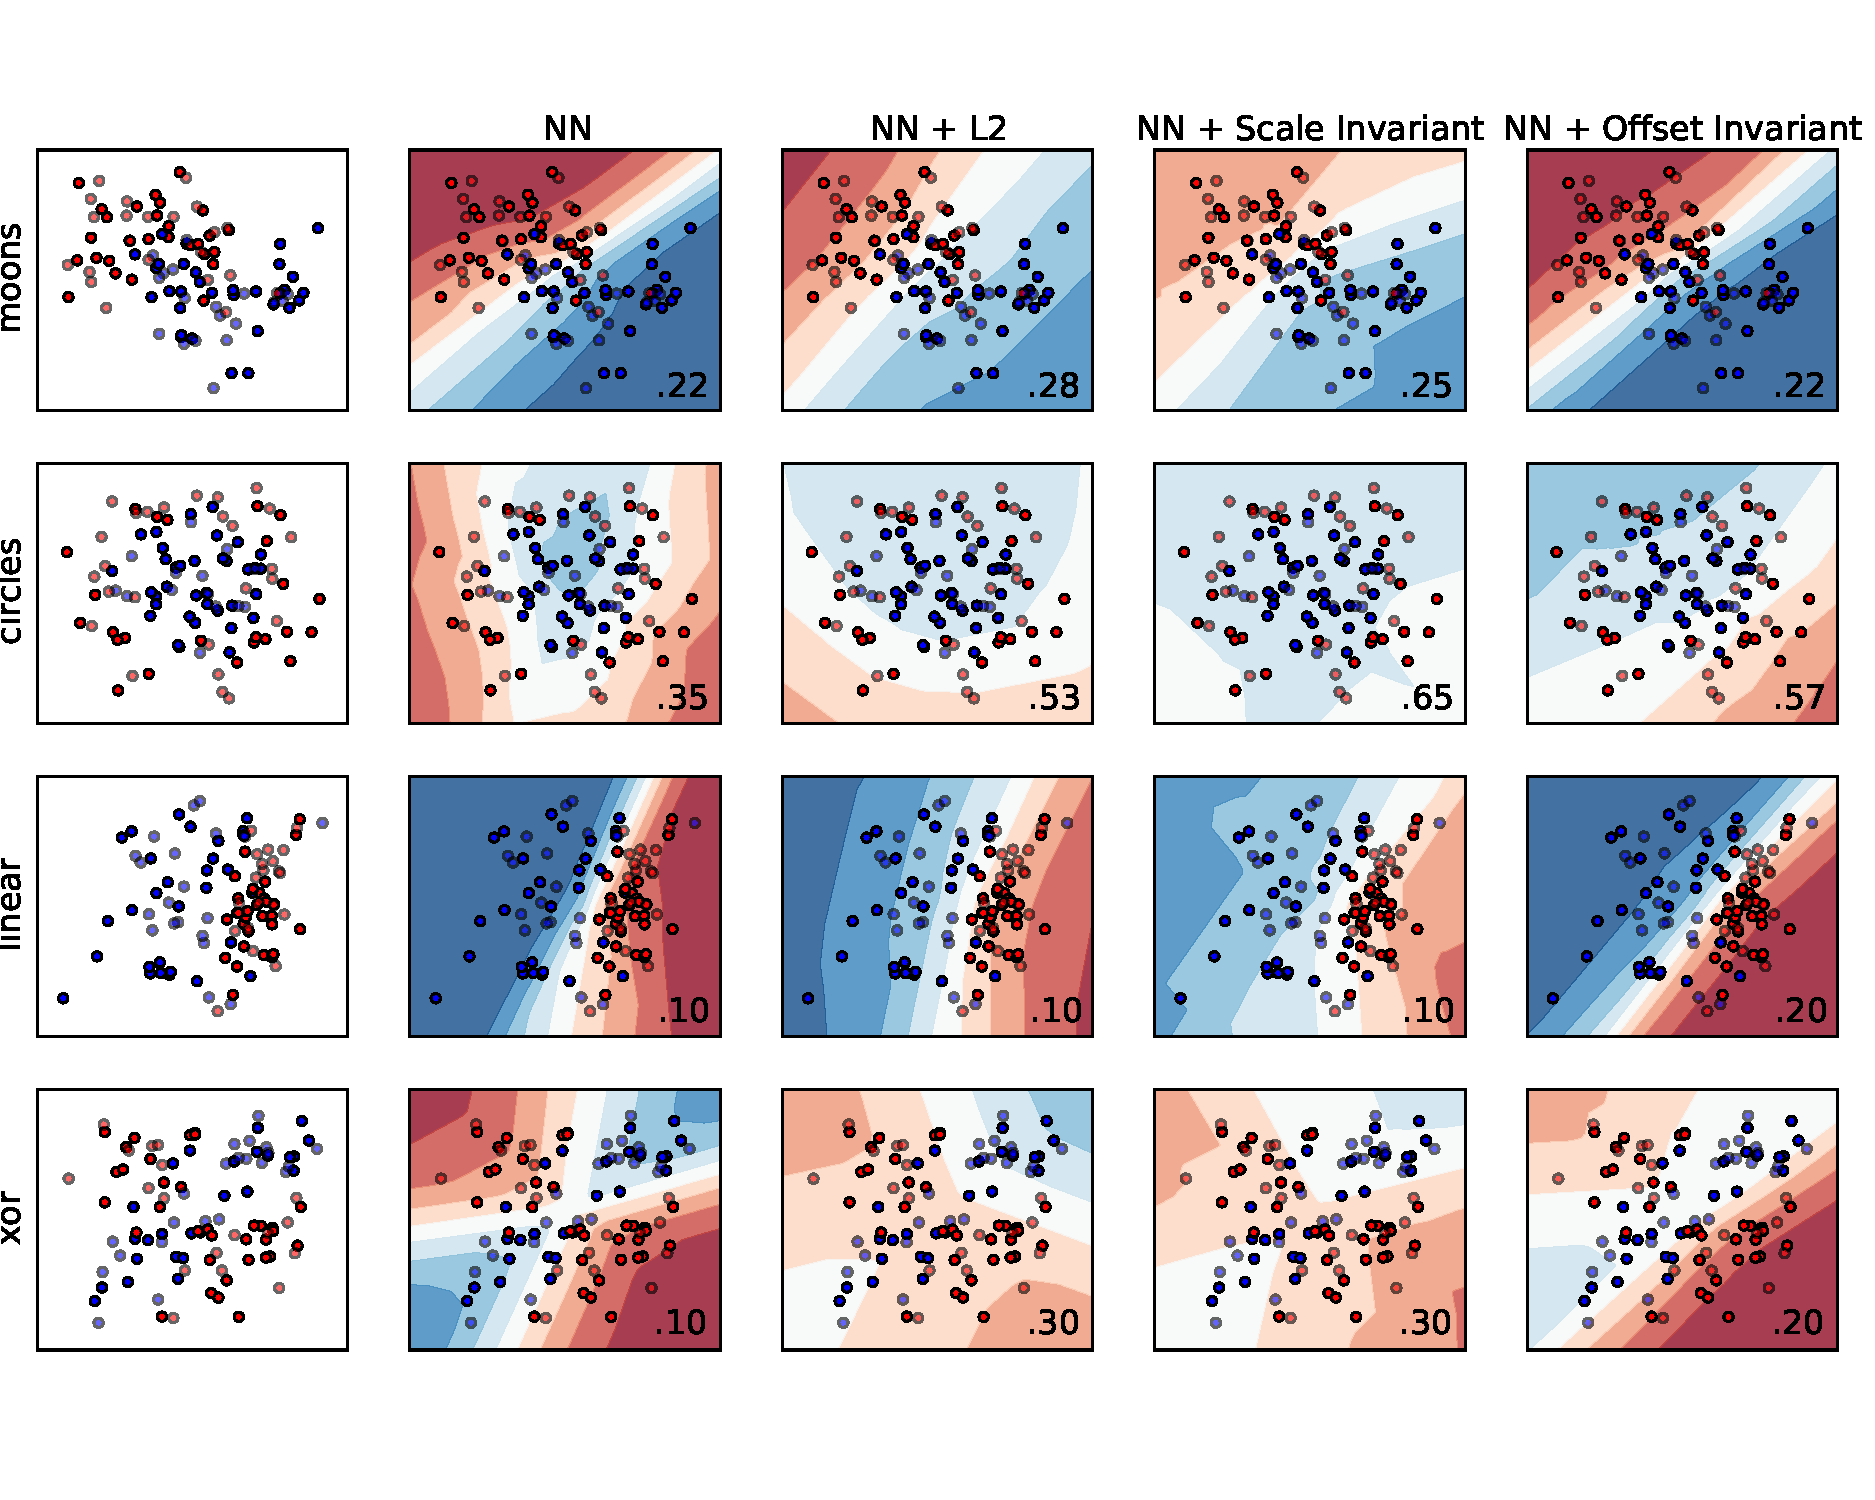
\includegraphics[width=0.7\textwidth, trim = 0 2.2cm 0 2cm, clip]{plots/2d_classifier}
	\caption{Observations and contour plot of the class probability function for each classifier and dataset.}
\end{figure*}

100 datasets for each data generator was then created to determine if are any statistical difference in the performance.

\begin{figure}[H]
	\centering
	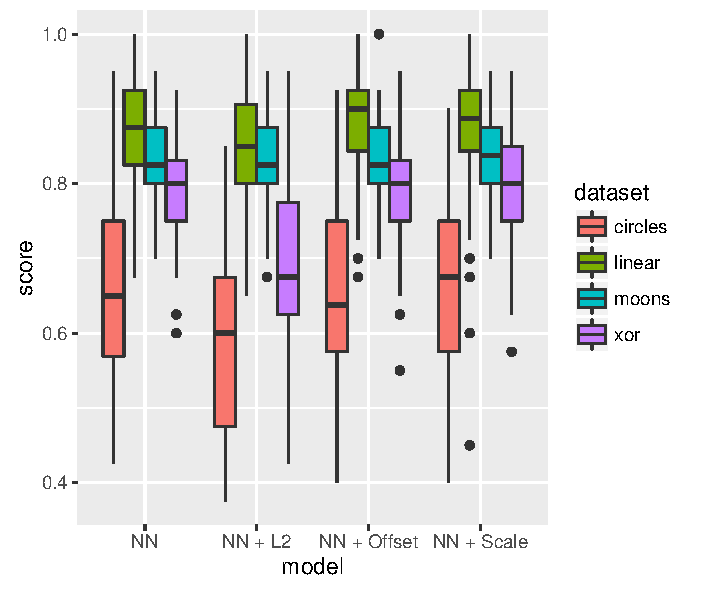
\includegraphics[width=0.5\textwidth]{plots/2d_significant}
	\caption{Boxplot of performance on the 100 datasets for each data generator and classification model.}
\end{figure}

In order to test whether weight decay has an significant improvement to the performance, an independent two-sampled t-test is used (assumes equal variance) on the misclassification rates obtained from the $5$-fold cross-validation for different weight decay parameter values seen in \cref{fig:reg_opt}.

\begin{figure}[H]
  \centering
  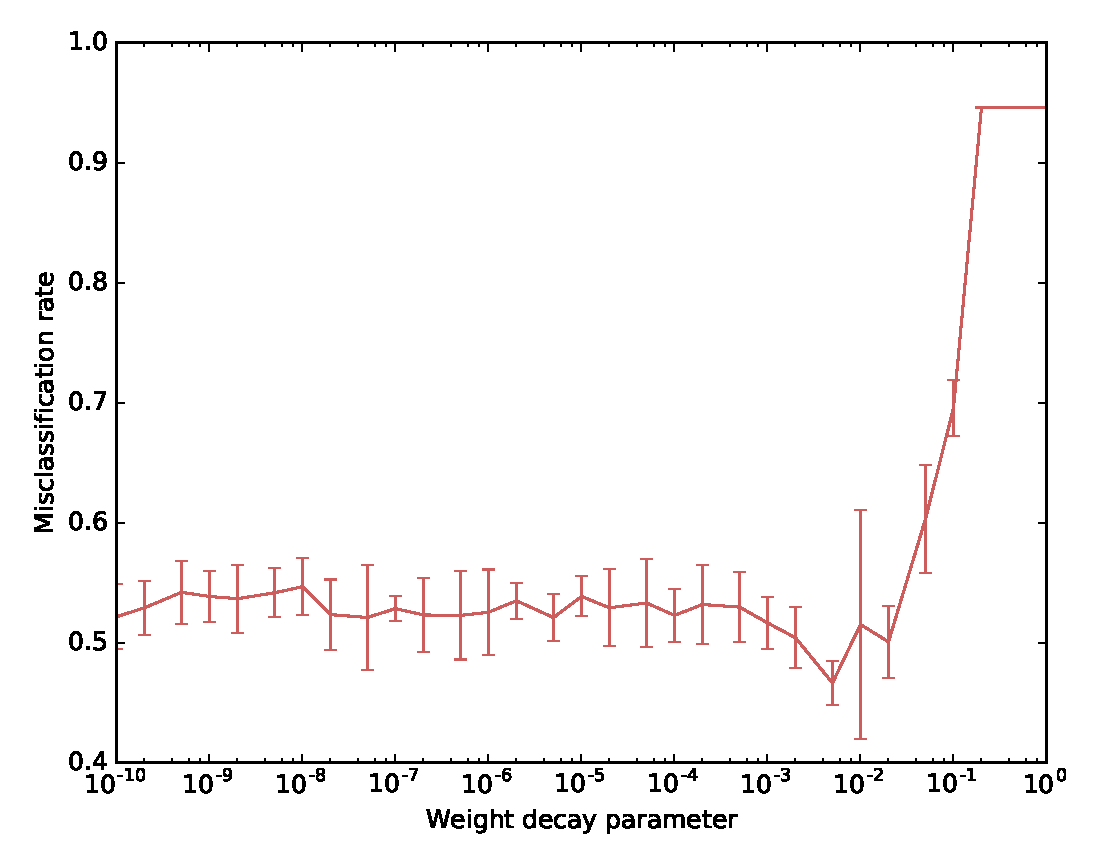
\includegraphics[width=0.4\textwidth]{plots/reg_opt_dieleman_speaker_elsdsr}
  \caption{Misclassification rate confidence interval for different weight decay parameter values, for the speaker classification problem on the ELSDSR dataset, obtained using $5$-fold cross-validation.}
  \label{fig:reg_opt}
\end{figure}

Given the mean misclassification rates $\mu_1$ and $\mu_2$ for the regularization parameter being $0$ and $5 \cdot 10^{-3}$ respectively, our null-hypothesis is defined as $\mu_1$ and $\mu_2$ being different
\begin{equation}
\begin{aligned}
\text{H}_\text{0} \, &\text{:} \, \mu_1 \ne \mu_2 \\
\text{H}_\text{a} \, &\text{:} \, \mu_1 = \mu_2.
\end{aligned}
\end{equation}
The resulting p-value for a two-sided t-test is $p = 0.0030$ i.e. the null-hypothesis is rejected and our alternative hypothesis is confirmed, hence we cannot say that adding weight decay has significant performance improvement with a $95\%$ significance level.


•Objective presentation of key results, without interpretation (text and tables
and figures)
•Important negative results should also be reported
